% Micaela Marais's protected main-slide section begins here.
\speakerlabel{Micaela}{1:10}
\begin{frame}{The learned hedge has the right financial shape}
  \begin{columns}[T,onlytextwidth]
    \begin{column}{0.71\textwidth}
      \begin{tikzpicture}[x=2.25cm,y=1cm]
        \draw[-{Latex[length=2mm]},line width=0.9pt,color=Slate] (0,0)--(3.25,0);
        \foreach \x in {0.3,1.6,2.9}
          \draw[Slate] (\x,-0.08)--(\x,0.08);
        \node[below,font=\scriptsize,color=Slate] at (0.3,-0.08) {deep OTM};
        \node[below,font=\scriptsize,color=Slate] at (1.6,-0.08) {near strike};
        \node[below,font=\scriptsize,color=Slate] at (2.9,-0.08) {deep ITM};

        \node[rounded corners=4pt,fill=Mist,minimum width=1.55cm,minimum height=1.35cm,
          align=center] at (0.3,1.05) {{\color{Teal}\Large\(\delta\to0\)}\\[-0.05cm]\scriptsize little stock needed};
        \node[rounded corners=4pt,fill=Gold!12,minimum width=1.55cm,minimum height=1.35cm,
          align=center] at (1.6,1.05) {{\color{Gold!80!black}\Large\(\nearrow\)}\\[-0.05cm]\scriptsize smooth transition};
        \node[rounded corners=4pt,fill=Teal!12,minimum width=1.55cm,minimum height=1.35cm,
          align=center] at (2.9,1.05) {{\color{Teal}\Large\(\delta\to1\)}\\[-0.05cm]\scriptsize nearly one-for-one};
        \draw[-{Latex[length=2mm]},line width=1.4pt,color=Teal]
          (0.62,1.05) .. controls (1.15,1.05) and (1.15,1.38) .. (1.32,1.38);
        \draw[-{Latex[length=2mm]},line width=1.4pt,color=Teal]
          (1.88,1.38) .. controls (2.05,1.38) and (2.05,1.05) .. (2.58,1.05);
      \end{tikzpicture}
    \end{column}
    \begin{column}{0.25\textwidth}
      \begin{tightitemize}
        \item monotone in moneyness;
        \item close to both analytic curves;
        \item nearly indistinguishable on representative OTM, ATM and ITM paths.
      \end{tightitemize}
    \end{column}
  \end{columns}
  \vspace{0.18cm}
  \claimbox{The network learned the expected hedge function, not only a low aggregate loss.}
  \sourcefoot{Economic reading of submitted report Figures 3.3 and 3.5; schematic above is not a data redraw.}
  \note{Use the three moneyness regimes to explain the hedge. Refer to the submitted report figures if an examiner asks for path-level evidence.}
\end{frame}



\speakerlabel{Micaela}{1:30}
\begin{comment}
    
\begin{frame}[t]{Parameter Robustness under Retraining}
  \vspace{-0.3cm}
  \begin{center}
    \footnotesize
    One-factor-at-a-time retraining around baseline $(K,\sigma,T,N) = (0.9, 0.4, 0.5, 125)$
    \vspace{0.05cm}

    $K \in \{0.8, 0.9, 1.0, 1.1, 1.2\} \qquad \sigma \in \{0.2, 0.4, 0.6\} \qquad
     T \in \{0.25, 0.5, 1.0\} \qquad N \in \{30, 60, 125, 250\}$
  \end{center}
  \vspace{0.2cm}
  \begin{columns}[c,onlytextwidth]
    \begin{column}{0.56\textwidth}
      \centering
      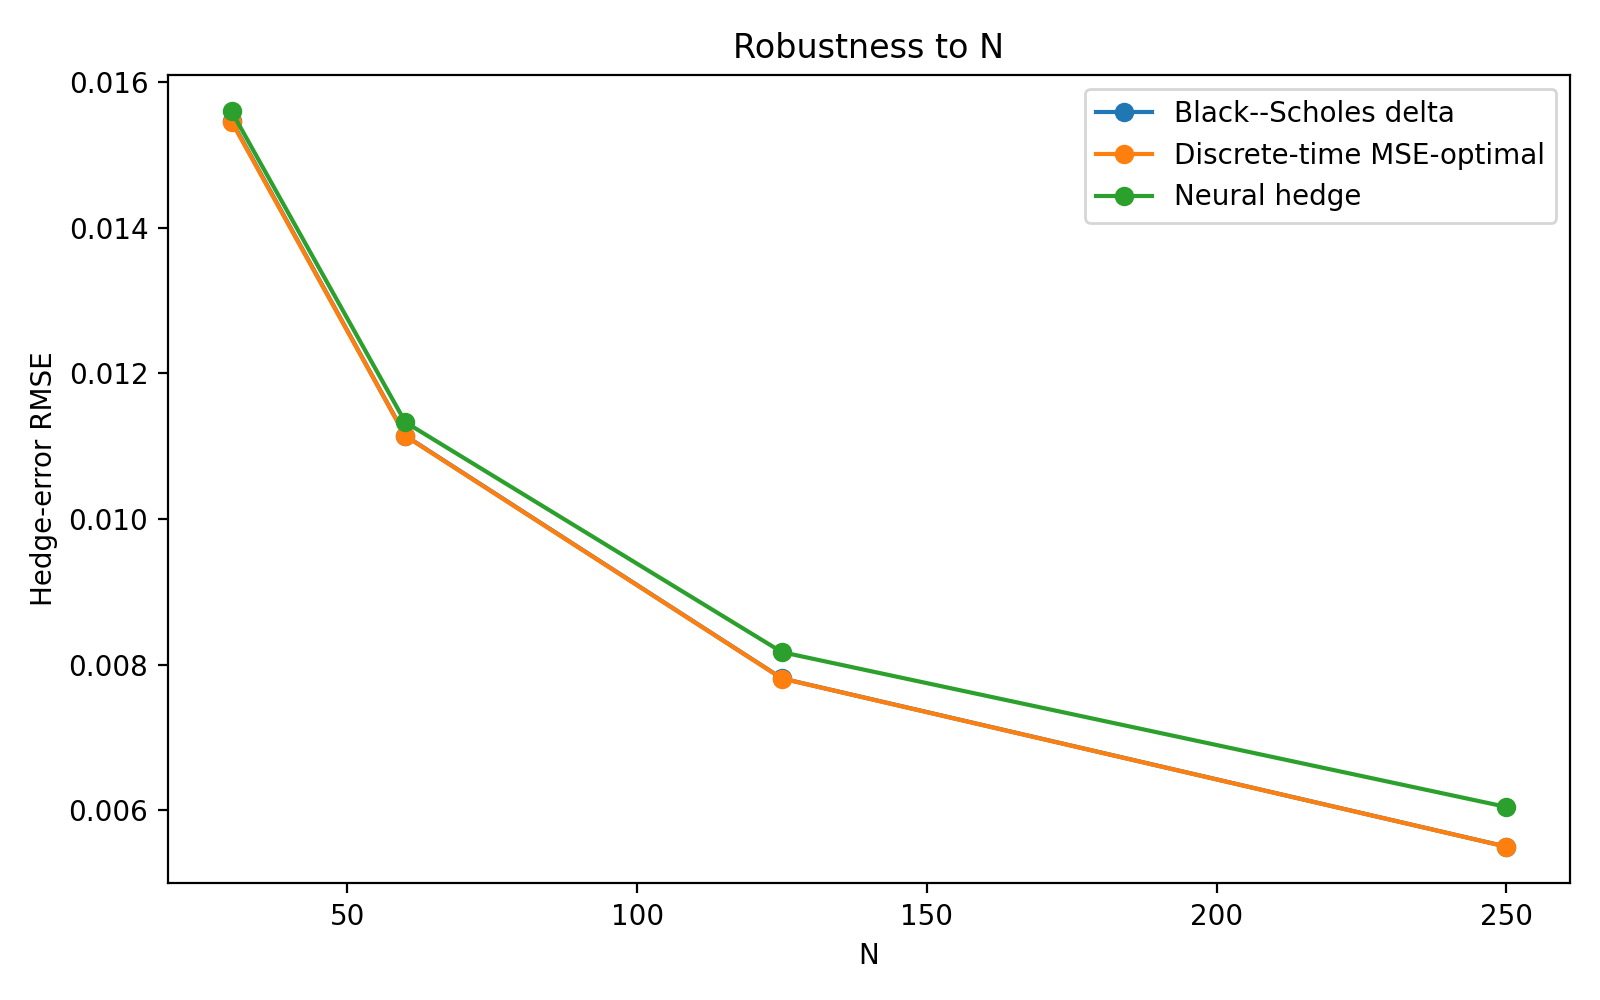
\includegraphics[width=0.85\linewidth]{sections/robustness_rmse_vs_N.png}
    \end{column}
    \begin{column}{0.4\textwidth}
      \centering
      {\color{Coral}\fontsize{20}{22}\selectfont\bfseries 3--8\%\par}
      {\small\color{DeepNavy} above DT-optimal, across all tested settings\par}
      \vspace{0.4cm}
      {\color{Coral}\fontsize{20}{22}\selectfont\bfseries 1.049\par}
      {\small\color{DeepNavy} mean NN/DT ratio (range 1.009--1.099)\par}
      \vspace{0.4cm}
      {\color{Coral}\fontsize{16}{18}\selectfont\bfseries $>$10$\times$ tighter\par}
      {\small\color{DeepNavy} than the degree-2 polynomial baseline\par}
    \end{column}
  \end{columns}
  \vfill
  \sourcefoot{Submitted report, Sec.\ 4.1.1, Table 4.1 and Figure 4.1.}
\end{frame}

\begin{frame}{\fontsize{16}{18}\selectfont Generalization Failure of the Single-Scenario Hedger}
  \centering
  \begin{tikzpicture}
    \begin{axis}[
      width=0.98\textwidth, height=5.8cm,
      ybar, bar width=10pt,
      ymin=0, ymax=320,
      ylabel={RMSE Ratio To Discrete-Time MSE-Optimal Benchmark},
      ylabel style={font=\scriptsize, color=DeepNavy},
      ytick={0,50,100,150,200,250,300},
      yticklabel style={font=\scriptsize, color=Slate},
      axis lines*=left,
      axis line style={color=Slate},
      ymajorgrids, grid style={color=Mist, line width=0.4pt},
      symbolic x coords={K0.9s0.4,K0.9s0.6,K1.1s0.6,K1.1s0.4,K0.9s0.2,K0.7s0.6,K1.1s0.2,K0.7s0.4,K0.7s0.2},
      xtick=data,
      xticklabels={{$K{=}0.9,\sigma{=}0.4^\ast$},{$K{=}0.9,\sigma{=}0.6$},{$K{=}1.1,\sigma{=}0.6$},{$K{=}1.1,\sigma{=}0.4$},{$K{=}0.9,\sigma{=}0.2$},{$K{=}0.7,\sigma{=}0.6$},{$K{=}1.1,\sigma{=}0.2$},{$K{=}0.7,\sigma{=}0.4$},{$K{=}0.7,\sigma{=}0.2$}},
      xticklabel style={rotate=90, anchor=east, font=\tiny, color=DeepNavy, inner sep=1pt},
      enlarge x limits=0.07,
      nodes near coords={\pgfmathprintnumber[precision=1,fixed]{\pgfplotspointmeta}x},
      every node near coord/.append style={font=\scriptsize, color=DeepNavy, anchor=south},
      tick style={draw=none},
    ]
      \addplot[ybar, fill=Coral, draw=none] coordinates {
        (K0.9s0.6,4.8) (K1.1s0.6,7.8) (K1.1s0.4,14.1) (K0.9s0.2,14.3)
        (K0.7s0.6,24.7) (K1.1s0.2,39.3) (K0.7s0.4,40.6) (K0.7s0.2,291.3)
      };
      \addplot[ybar, fill=Teal, draw=none] coordinates {(K0.9s0.4,1.0)};
    \end{axis}
  \end{tikzpicture}
  \sourcefoot{Submitted report, Table 4.2. Single-scenario hedger evaluated without retraining across strike ($K$) and volatility ($\sigma$) combinations; ratio is neural hedge RMSE to discrete-time MSE-optimal RMSE.}
\end{frame}



\begin{frame}{Parameter-Conditioned Hedger}
  \vspace{-0.2cm}
  \begin{center}
    \[
      \delta_n = f_\theta\!\left(\log\frac{S_{t_n}}{K},\ \frac{\tau_n}{T},\ K,\ \sigma\right)
    \]
    \vspace{-0.25cm}
    $K \sim U(0.7, 1.1) \qquad \sigma \sim U(0.2, 0.6)$
  \end{center}
  \vspace{0.15cm}
  \begin{beamercolorbox}[rounded=true,sep=0.35cm]{block body}
    \begin{columns}[c,onlytextwidth]
      \begin{column}{0.48\textwidth}
        \begin{table}
          \centering
          \scriptsize
          \setlength{\tabcolsep}{4pt}
          \begin{tabular}{lS[table-format=1.1]S[table-format=1.1]S[table-format=1.6]S[table-format=1.6]}
            \toprule
            Region & {$K$} & {$\sigma$} & {DT} & {NN}\\
            \midrule
            Interp. & 0.9 & 0.4 & 0.007813 & 0.007830\\
            Interp. & 1.1 & 0.6 & 0.013715 & 0.013783\\
            Extrap. & 0.6 & 0.4 & 0.002220 & 0.002241\\
            Extrap. & 0.9 & 0.1 & 0.001019 & 0.003404\\
            Extrap. & 1.3 & 0.8 & 0.019187 & 0.020058\\
            \bottomrule
          \end{tabular}
        \end{table}
        \vspace{0.3cm}
        \scriptsize\color{DeepNavy}
        Each path uses its analytic Black--Scholes premium --- pricing is separated from hedging.
      \end{column}
      \begin{column}{0.46\textwidth}
        \centering
        {\color{Coral}\fontsize{15}{17}\selectfont\bfseries \(\leq\)0.00018\par}
        {\scriptsize\color{DeepNavy} max.\ RMSE gap, all 9 interpolation points\par}
        \vspace{0.22cm}
        {\color{Coral}\fontsize{15}{17}\selectfont\bfseries \(\leq\)0.00004\par}
        {\scriptsize\color{DeepNavy} strike-extrapolation RMSE gap\par}
        \vspace{0.22cm}
        {\color{Coral}\fontsize{15}{17}\selectfont\bfseries \(\sim\)3\(\times\)\par}
        {\scriptsize\color{DeepNavy} worst-case volatility-extrapolation gap}
      \end{column}
    \end{columns}
  \end{beamercolorbox}
  \vspace{0.15cm}
  \sourcefoot{Submitted report, Sec.\ 4.1.3, Table 4.3 and Algorithm A.6.3.}
\end{frame}


\begin{frame}{Parameter-Conditioned Hedger vs.\ Retraining}

\begin{table}[h]
\centering
\scriptsize
\setlength{\tabcolsep}{4pt}
\begin{tabular}{cccc S[table-format=1.6] S[table-format=1.6] S[table-format=1.6] S[table-format=1.3] S[table-format=1.3]}
\toprule
$K$ & $\sigma$ & $T$ & $N$ & {DT-opt RMSE} & {Retrained NN} & {Param-cond NN} & {Retr.\ NN/DT} & {PC NN/DT} \\
\midrule
0.9 & 0.2 & 0.5 & 125 & 0.003400 & 0.003680 & 0.003492 & 1.082 & 1.026 \\
0.9 & 0.4 & 0.5 & 125 & 0.007810 & 0.008172 & 0.007830 & 1.046 & 1.002 \\
0.9 & 0.6 & 0.5 & 125 & 0.011827 & 0.012334 & 0.011891 & 1.043 & 1.003 \\
1.1 & 0.4 & 0.5 & 125 & 0.008983 & 0.009248 & 0.009071 & 1.030 & 1.003 \\
\bottomrule
\end{tabular}
\caption{\scriptsize Comparison at the four shared $(K,\sigma,T,N)$ settings between Table 4.1 (retraining) and Table 4.3 (parameter-conditioned).}
\end{table}

\vspace{0.5em}
\begin{columns}[T]
\begin{column}{0.48\textwidth}
\textbf{\small Summary statistics}
\begin{itemize}
\scriptsize
\item Mean NN/DT ratio: \textbf{1.050} (retrained) vs.\ \textbf{1.009} (param-cond)
\item Mean excess RMSE above DT-optimal: \textbf{0.000354} vs.\ \textbf{0.000066}
\item Param-cond beats retrained on RMSE in \textbf{4/4} settings tested
\end{itemize}
\end{column}
\begin{column}{0.48\textwidth}
\textbf{\small Training time}
\begin{itemize}
\scriptsize
\item Param-conditioned: \textbf{433s} (one run)
\item Retraining (combined): \textbf{992s} (per-scenario)
\item Covers a \emph{continuous} $(K,\sigma)$ range vs.\ fixed points
\end{itemize}
\end{column}
\end{columns}

\end{frame}





\begin{frame}[t]{Parameter Robustness under Retraining}
  \vspace{-0.3cm}
  \begin{center}
    \footnotesize
    Same architecture, \textbf{retrained from scratch} at each setting
    (one factor at a time) around baseline
    $(K,\sigma,T,N)=(0.9,\,0.4,\,0.5,\,125)$.\\[0.12cm]
    $K \in \{0.8, 0.9, 1.0, 1.1, 1.2\}
    \qquad
    \sigma \in \{0.2, 0.4, 0.6\}
    \qquad
    T \in \{0.25, 0.5, 1.0\}
    \qquad
    N \in \{30, 60, 125, 250\}$
  \end{center}
  \vspace{0.05cm}
  \begin{columns}[c,onlytextwidth]
    %------------------------------------------------
    % Left column: key statistics
    %------------------------------------------------
    \begin{column}{0.46\textwidth}
      \centering
      {\color{Coral}
      \fontsize{15}{17}\selectfont
      \bfseries
      1.049
      \par}
      \vspace{0.12cm}
      {\footnotesize\color{DeepNavy}
      Mean NN/DT ratio (range 1.009--1.099)
      \par}
      \vspace{0.40cm}
      {\color{Coral}
      \fontsize{15}{17}\selectfont
      \bfseries
      \boldmath$\leq$\unboldmath\,10\%
      \par}
      \vspace{0.12cm}
      {\footnotesize\color{DeepNavy}
      Above DT-optimal, across all tested settings
      \par}
      \vspace{0.40cm}
      {\color{Coral}
      \fontsize{15}{17}\selectfont
      \bfseries
      N = 250
      \par}
      \vspace{0.12cm}
      {\footnotesize\color{DeepNavy}
      Worst case: benchmark shrinks faster than the network here
      \par}
    \end{column}
    %------------------------------------------------
    % Right column: graph
    %------------------------------------------------
    \begin{column}{0.51\textwidth}
      \centering
      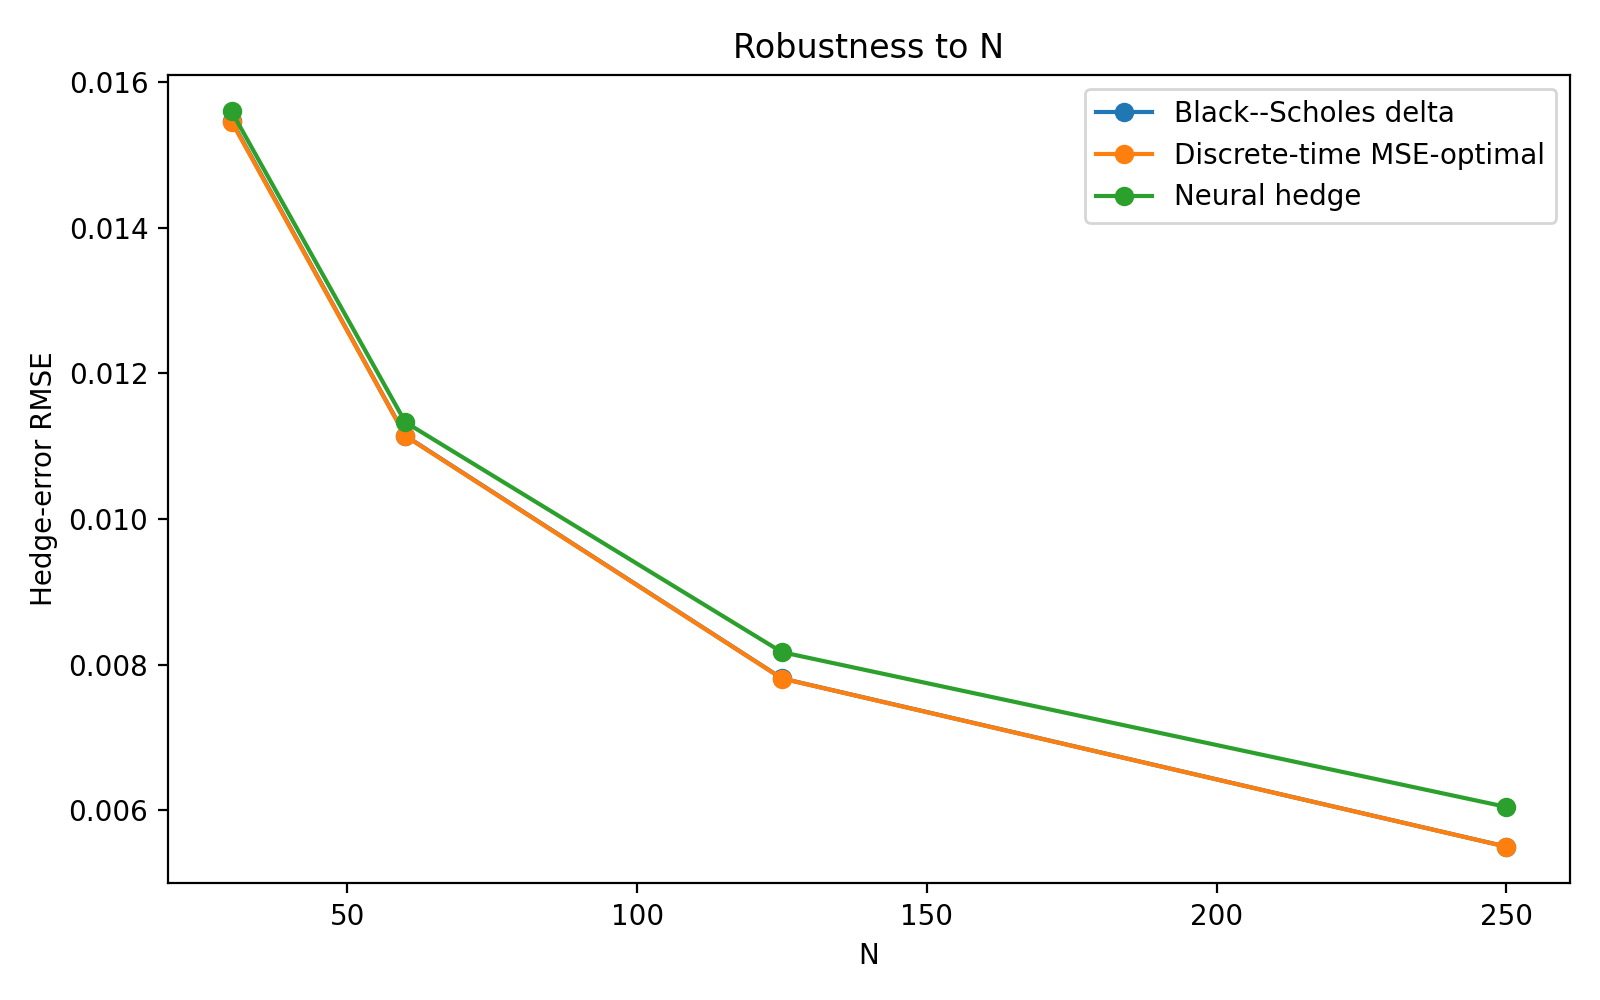
\includegraphics[
        width=0.98\linewidth
      ]{sections/robustness_rmse_vs_N.png}
    \end{column}
  \end{columns}
  \vfill
  \sourcefoot{Submitted report, Sec.\ 4.1.1, Table 4.1 and Figure 4.1.}
\end{frame}

\end{comment}

\begin{comment}
    
\begin{frame}[t]{Parameter Robustness under Retraining}
  \vspace{-0.3cm}

  \begin{center}
    \footnotesize
    Same architecture, \textbf{retrained from scratch} at each setting (one factor at a time)
    around baseline $(K,\sigma,T,N) = (0.9,\,0.4,\,0.5,\,125)$.\\[0.15cm]

    $K \in \{0.8, 0.9, 1.0, 1.1, 1.2\} \qquad
    \sigma \in \{0.2, 0.4, 0.6\} \qquad
    T \in \{0.25, 0.5, 1.0\} \qquad
    N \in \{30, 60, 125, 250\}$
  \end{center}

  \vspace{0.2cm}

  \begin{columns}[c,onlytextwidth]

    \begin{column}{0.56\textwidth}
      \centering
      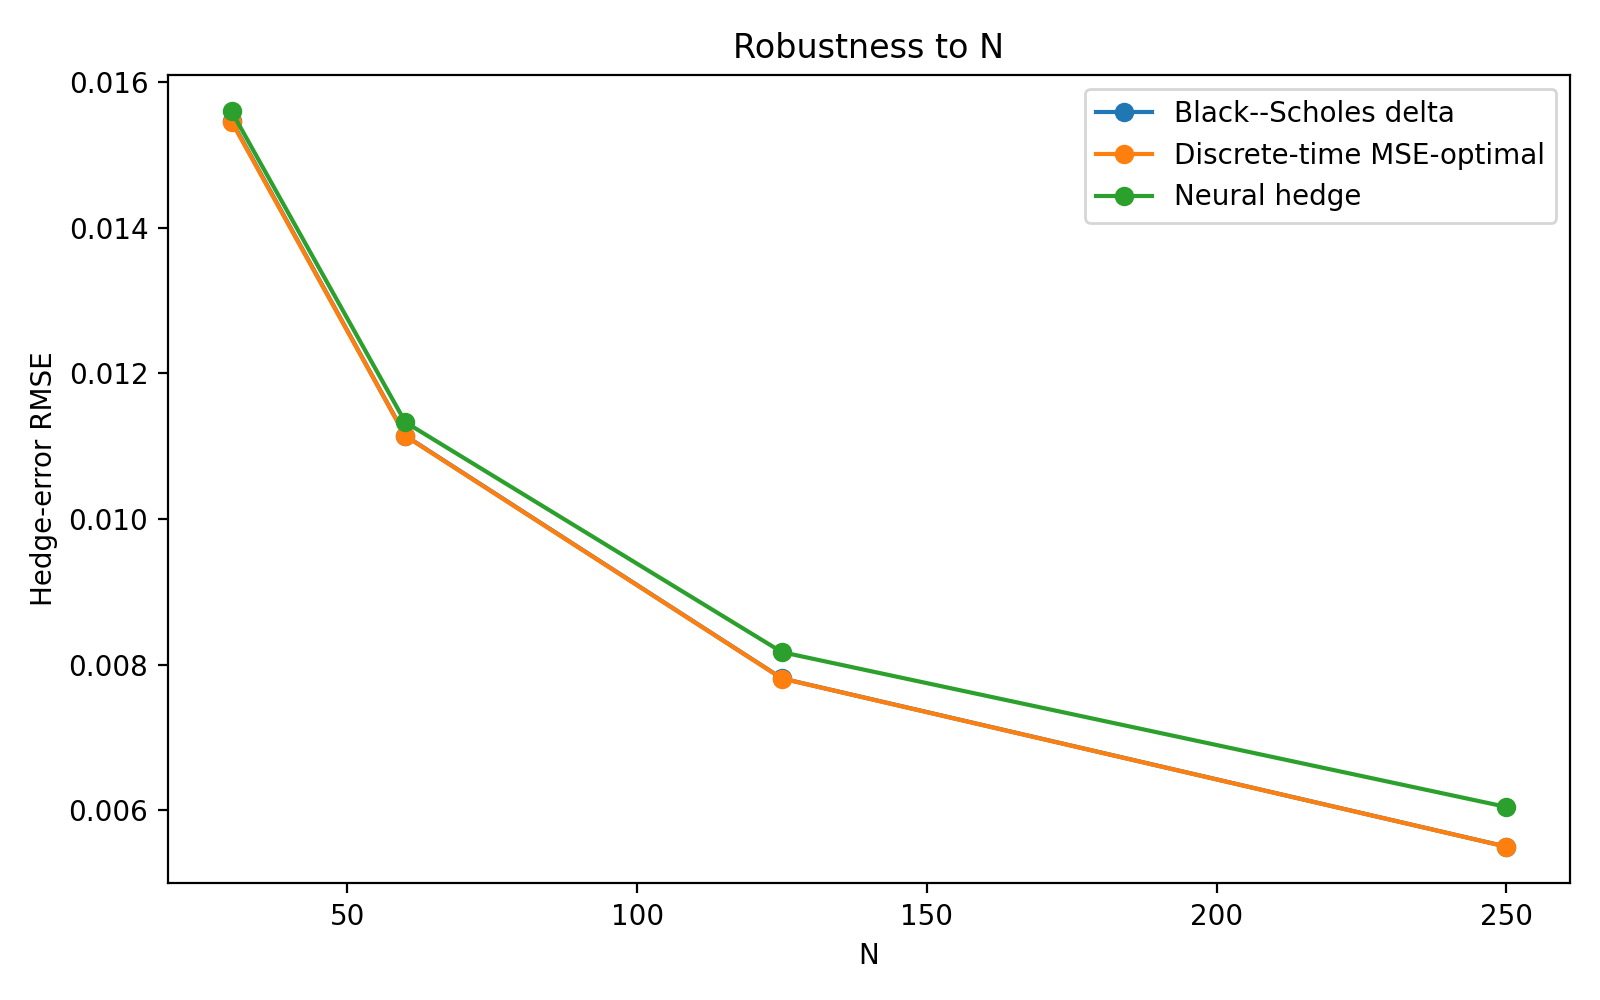
\includegraphics[width=0.85\linewidth]{sections/robustness_rmse_vs_N.png}
    \end{column}

    \begin{column}{0.40\textwidth}
      \centering

      {\color{Coral}\fontsize{20}{22}\selectfont\bfseries 3--10\%\par}
      {\small\color{DeepNavy}Above DT-optimal, across all tested settings\par}

      \vspace{0.4cm}

      {\color{Coral}\fontsize{20}{22}\selectfont\bfseries 1.049\par}
      {\small\color{DeepNavy}Mean NN/DT ratio (range 1.009--1.099)\par}

      \vspace{0.4cm}

      {\color{Coral}\fontsize{16}{18}\selectfont\bfseries $\approx$184\%\par}
      {\small\color{DeepNavy}Above optimal for the degree-2 polynomial\par}

    \end{column}

  \end{columns}

  \vfill
  \sourcefoot{Submitted report, Sec.\ 4.1.1, Table 4.1 and Figure 4.1.}
\end{frame}

\end{comment}
 
% ---------------------------------------------------------------------
% SLIDE 7 : Generalization Failure  (unchanged from v1 -- included for completeness)
% ---------------------------------------------------------------------

\begin{comment}
    
\speakerlabel{Micaela}{1:30}
\begin{frame}{\fontsize{15}{17}\selectfont Generalization Failure of the Single-Scenario Hedger}
  \vspace{-0.08cm}
  \begin{center}
    {\footnotesize One model \textbf{trained once} at $(K^\ast,\sigma^\ast)=(0.9,0.4)$,
     evaluated elsewhere \textbf{without retraining}.}
  \end{center}
  \vspace{-0.02cm}
  \begin{columns}[c,onlytextwidth]
    \begin{column}{0.6\textwidth}
      \centering
      \begin{tikzpicture}
        \begin{axis}[
          width=\linewidth, height=5.2cm,
          ybar, bar width=8pt,
          ymin=0, ymax=320,
          ylabel={NN/DT RMSE Ratio},
          ylabel style={font=\scriptsize,color=DeepNavy},
          ytick={0,50,100,150,200,250,300},
          yticklabel style={font=\scriptsize,color=Slate},
          axis lines*=left, axis line style={color=Slate},
          ymajorgrids, grid style={color=Mist,line width=0.4pt},
          symbolic x coords={K0.9s0.4,K0.9s0.6,K1.1s0.6,K1.1s0.4,K0.9s0.2,K0.7s0.6,K1.1s0.2,K0.7s0.4,K0.7s0.2},
          xtick={K0.9s0.4,K0.9s0.6,K1.1s0.6,K1.1s0.4,K0.9s0.2,K0.7s0.6,K1.1s0.2,K0.7s0.4,K0.7s0.2},
          xticklabels={{$0.9,0.4^\ast$},{$0.9,0.6$},{$1.1,0.6$},{$1.1,0.4$},{$0.9,0.2$},{$0.7,0.6$},{$1.1,0.2$},{$0.7,0.4$},{$0.7,0.2$}},
          xticklabel style={rotate=90,anchor=east,font=\tiny,color=DeepNavy,inner sep=1pt},
          enlarge x limits=0.07,
          nodes near coords={\pgfmathprintnumber[precision=1,fixed]{\pgfplotspointmeta}$\times$},
          every node near coord/.append style={font=\tiny,color=DeepNavy,anchor=south},
          tick style={draw=none},
        ]
          \addplot[ybar,fill=Coral,draw=none] coordinates {
            (K0.9s0.6,4.8)(K1.1s0.6,7.8)(K1.1s0.4,14.1)(K0.9s0.2,14.3)
            (K0.7s0.6,24.7)(K1.1s0.2,39.3)(K0.7s0.4,40.6)(K0.7s0.2,291.3)};
          \addplot[ybar,fill=Teal,draw=none] coordinates {(K0.9s0.4,1.0)};
        \end{axis}
      \end{tikzpicture}
      \\[0.02cm]
      {\scriptsize\color{Slate} $x$-axis: $(K,\sigma)$ pairs.}
    \end{column}
    \begin{column}{0.38\textwidth}
      \pill[Coral]{Why it fails}
      \vspace{0.14cm}
 
      {\scriptsize
       \textbf{1.\ One scenario.} Trained on a single fixed $(K^\ast,\sigma^\ast)$ --- no variation to learn parameter dependence from.\par\vspace{0.14cm}
       \textbf{2.\ Strike hardcoded.} $K^\ast$ is baked into log-moneyness, so a new strike feeds the network the \emph{wrong} number, not merely an unseen one.\par\vspace{0.14cm}
       \textbf{3.\ No $\sigma$ input.} Volatility is absent, so the network can't detect that market conditions have changed --- it just reapplies whatever it learned at $\sigma^\ast$, regardless of the true volatility.\par}
    \end{column}
  \end{columns}
  \vspace{0.05cm}
  \sourcefoot{Submitted report, Sec.\ 4.1.2, Table 4.2. }
  \note{Contrast with the previous slide: there the architecture was retrained per setting and stayed within 3--8\%; here the SAME architecture is frozen and fails by up to two orders of magnitude. The three causes compound --- fixing only one would not help. Worst case $(0.7,0.2)$: RMSE jumps from $0.0005$ to $0.14$.}
\end{frame}


\end{comment}

\begin{comment}
\speakerlabel{Micaela}{1:30}
\begin{frame}{Parameter-Conditioned Hedger}
  \begin{columns}[T,onlytextwidth]
    \begin{column}{0.48\textwidth}
      \begin{beamercolorbox}[rounded=true,sep=0.24cm]{block body}
        \pill{Original}
        \vspace{0.14cm}
        {\small
        \begin{tightitemize}
          \item \textbf{Inputs:} $(\log(S/K),\ \tau/T)$
          \item \textbf{Training:} Fixed $K=0.9$, $\sigma=0.4$
          \item \textbf{Paths:} 100k
          \item \textbf{Pricing:} Learned premium
        \end{tightitemize}}
      \end{beamercolorbox}
    \end{column}
    \begin{column}{0.48\textwidth}
      \begin{beamercolorbox}[rounded=true,sep=0.24cm]{block body}
        \pill{Conditioned}
        \vspace{0.14cm}
        {\small
        \begin{tightitemize}
          \item \textbf{Inputs:} $(\log(S/K),\ \tau/T,\ K,\ \sigma)$
          \item \textbf{Training:} $K\sim U(0.7,1.1)$, $\sigma\sim U(0.2,0.6)$
          \item \textbf{Paths:} 200k
          \item \textbf{Pricing:} Analytic BS premium
        \end{tightitemize}}
      \end{beamercolorbox}
    \end{column}
  \end{columns}
  \vspace{0.28cm}
  \begin{columns}[T,onlytextwidth]
    \begin{column}{0.48\textwidth}
      \centering
      \pill{Interpolation}
      \par\vspace{0.14cm}
      {\small Inside trained range:\\
      $K\in[0.7,1.1]$, $\sigma\in[0.2,0.6]$\par}
      \vspace{0.22cm}
      {\small\color{DeepNavy} Max RMSE gap across all 9 test scenarios\par}
      \vspace{0.08cm}
      {\small\color{Coral}\bfseries \boldmath$\leq$\unboldmath\,0.00018\par}
    \end{column}
    \begin{column}{0.48\textwidth}
      \centering
      \pill{Extrapolation}
      \par\vspace{0.14cm}
      {\small Outside trained range:\\
      $K\in\{0.6,1.3\}$, $\sigma\in\{0.1,0.8\}$\par}
      \vspace{0.22cm}
      {\small\color{DeepNavy}
      Strike RMSE stays within \textbf{\color{Coral}0.00004}\\[0.12cm]
      Worst vol.\ gap at $\sigma=0.1$: \textbf{\color{Coral}\boldmath$\approx$\unboldmath\,3\boldmath$\times$\unboldmath\ Optimal}\par}
    \end{column}
  \end{columns}
  \vspace{0.15cm}
  \sourcefoot{Submitted report, Sec.\ 4.1.3, Table 4.3.}
\end{frame}

\end{comment}

\begin{comment}
\begin{frame}[t]{Conditioning fixes the Generalisation Failure}

\vspace{-0.22cm}

%=================================================
% ORIGINAL VS CONDITIONED
%=================================================

\begin{beamercolorbox}[
    rounded=true,
    sep=0.22cm
]{block body}

\begin{columns}[T,onlytextwidth]

%-------------------------------------------------
% Original
%-------------------------------------------------
\begin{column}{0.455\textwidth}

\centering
\pill[DeepNavy]{Original}

\vspace{0.14cm}

\raggedright
{\footnotesize

\begin{itemize}
    \setlength{\itemsep}{0.16cm}
    \setlength{\parskip}{0pt}
    \setlength{\parsep}{0pt}
    \setlength{\leftmargini}{0.48cm}

    \item \textbf{Inputs:}\;
    $\bigl(\log(S/K),\,\tau/T\bigr)$

    \item \textbf{Training:}\;
    Fixed $K=0.9,\ \sigma=0.4$

    \item \textbf{Paths:}\;
    100k

    \item \textbf{Pricing:}\;
    Learned premium

\end{itemize}
}

\end{column}

%-------------------------------------------------
% Centre divider and arrow
%-------------------------------------------------
\begin{column}{0.07\textwidth}

\centering

\vspace{0.46cm}

{\color{Slate!45}\rule{0.5pt}{2.30cm}}

\vspace{-1.38cm}

{\color{DeepNavy}
\fontsize{20}{20}\selectfont
$\boldsymbol{\rightarrow}$}

\end{column}

%-------------------------------------------------
% Conditioned
%-------------------------------------------------
\begin{column}{0.455\textwidth}

\centering
\pill[Teal]{Conditioned}

\vspace{0.14cm}

\raggedright
{\footnotesize

\begin{itemize}
    \setlength{\itemsep}{0.16cm}
    \setlength{\parskip}{0pt}
    \setlength{\parsep}{0pt}
    \setlength{\leftmargini}{0.48cm}

    \item \textbf{Inputs:}\;
    $\bigl(\log(S/K),\,\tau/T,\,K,\,\sigma\bigr)$

    \item \textbf{Training:}\;
    $K\sim U(0.7,1.1),\;
    \sigma\sim U(0.2,0.6)$

    \item \textbf{Paths:}\;
    200k

    \item \textbf{Pricing:}\;
    Analytic BS premium

\end{itemize}
}

\end{column}

\end{columns}

\end{beamercolorbox}

\vspace{0.16cm}

%=================================================
% INTERPOLATION AND EXTRAPOLATION RESULTS
%=================================================

\begin{columns}[T,onlytextwidth]

%-------------------------------------------------
% Interpolation
%-------------------------------------------------
\begin{column}{0.49\textwidth}

\begin{beamercolorbox}[
    rounded=true,
    sep=0.22cm
]{block body}

\centering

\pill[Teal]{Interpolation}

\vspace{0.10cm}

{\small\color{DeepNavy}
Inside the trained range
\par}

\vspace{0.04cm}

{\footnotesize\color{Slate}
$K\in[0.7,1.1],\qquad
\sigma\in[0.2,0.6]$
\par}

\vspace{0.10cm}

{\color{Coral}
\fontsize{22}{23}\selectfont
\bfseries
$\leq 0.00018$
\par}

\vspace{0.07cm}

{\footnotesize\color{DeepNavy}
Maximum RMSE gap across all 9 test scenarios
\par}

\end{beamercolorbox}

\end{column}

\hfill

%-------------------------------------------------
% Extrapolation
%-------------------------------------------------
\begin{column}{0.49\textwidth}

\begin{beamercolorbox}[
    rounded=true,
    sep=0.22cm
]{block body}

\centering

\pill[Teal]{Extrapolation}

\vspace{0.10cm}

{\small\color{DeepNavy}
Outside the trained range
\par}

\vspace{0.04cm}

{\footnotesize\color{Slate}
$K\in\{0.6,1.3\},\qquad
\sigma\in\{0.1,0.8\}$
\par}

\vspace{0.10cm}

{\color{Coral}
\fontsize{22}{23}\selectfont
\bfseries
$\sim 3\times$
\par}

\vspace{0.07cm}

{\footnotesize\color{DeepNavy}
Worst volatility gap at $\sigma=0.1$;\\
strike extrapolation remains within $0.00004$
\par}

\end{beamercolorbox}

\end{column}

\end{columns}

\vspace{0.15cm}

%=================================================
% TRAINING-TIME CLAIM
%=================================================

\begin{beamercolorbox}[
    rounded=true,
    sep=0.18cm
]{block body}

\centering

{\small\bfseries\color{DeepNavy}
One
{\color{Teal}433\,s}
training run covers the full $(K,\sigma)$ range
\textemdash\\[-0.01cm]
versus
{\color{Teal}992\,s}
combined to retrain separately for each individual setting.
}

\end{beamercolorbox}

\vspace{0.06cm}

%=================================================
% SOURCE
%=================================================

{\tiny\color{Slate}
Submitted report, Sec.\ 4.1.3, Table 4.3;
efficiency comparison with Table 4.1.
}

\note{
The comparison at the top shows exactly how the original model was
changed. Strike and volatility were added as inputs, the network was
trained across a continuous range of contract settings, the number of
training paths was increased, and the analytic Black--Scholes premium
was supplied so that the experiment isolates hedging performance rather
than pricing. The conditioned network performs very well within the
training range, remains robust when extrapolating in strike, and only
shows a material deterioration when extrapolating to very low
volatility.
}

\end{frame}







\begin{frame}[t]{Conditioning fixes the Generalisation Failure}

\vspace{-0.22cm}

%=================================================
% ORIGINAL VS CONDITIONED
%=================================================

\begin{beamercolorbox}[
    rounded=true,
    sep=0.16cm
]{block body}

\begin{columns}[T,onlytextwidth]

%-------------------------------------------------
% Original
%-------------------------------------------------
\begin{column}{0.465\textwidth}

\raggedright
\hspace{0.18cm}\pill[DeepNavy]{Original}

\vspace{0.07cm}

{\footnotesize
\begin{itemize}
    \setlength{\itemsep}{0.10cm}
    \setlength{\parskip}{0pt}
    \setlength{\parsep}{0pt}
    \setlength{\topsep}{0pt}
    \setlength{\partopsep}{0pt}
    \setlength{\leftmargini}{0.48cm}

    \item \textbf{Inputs:}\;
    $\bigl(\log(S/K),\,\tau/T\bigr)$

    \item \textbf{Training:}\;
    Fixed $K=0.9,\ \sigma=0.4$

    \item \textbf{Paths:}\;
    100k

    \item \textbf{Pricing:}\;
    Learned premium

\end{itemize}
}

\end{column}

%-------------------------------------------------
% Centre arrow
%-------------------------------------------------
\begin{column}{0.055\textwidth}

\centering

\vspace{1.18cm}

\raisebox{0pt}[0pt][0pt]{%
    \color{DeepNavy}%
    \makebox[0pt][c]{%
        \rule{0.43cm}{2.8pt}%
        \hspace{-0.4pt}%
        \raisebox{-0.11cm}{%
            \fontsize{18}{18}\selectfont
            $\blacktriangleright$%
        }%
    }%
}

\end{column}

%-------------------------------------------------
% Conditioned
%-------------------------------------------------
\begin{column}{0.465\textwidth}

\raggedright
\hspace{0.18cm}\pill[Teal]{Conditioned}

\vspace{0.07cm}

{\footnotesize
\begin{itemize}
    \setlength{\itemsep}{0.10cm}
    \setlength{\parskip}{0pt}
    \setlength{\parsep}{0pt}
    \setlength{\topsep}{0pt}
    \setlength{\partopsep}{0pt}
    \setlength{\leftmargini}{0.48cm}

    \item \textbf{Inputs:}\;
    $\bigl(\log(S/K),\,\tau/T,\,K,\,\sigma\bigr)$

    \item \textbf{Training:}\;
    $K\sim U(0.7,1.1),\;
    \sigma\sim U(0.2,0.6)$

    \item \textbf{Paths:}\;
    200k

    \item \textbf{Pricing:}\;
    Analytic BS premium

\end{itemize}
}

\end{column}

\end{columns}

\end{beamercolorbox}

\vspace{0.10cm}

%=================================================
% INTERPOLATION AND EXTRAPOLATION RESULTS
%=================================================

\begin{columns}[T,onlytextwidth]

%-------------------------------------------------
% Interpolation
%-------------------------------------------------
\begin{column}{0.49\textwidth}

\begin{beamercolorbox}[
    rounded=true,
    sep=0.20cm
]{block body}

\centering

\pill[Teal]{Interpolation}

\vspace{0.08cm}

{\small\color{DeepNavy}
Inside the trained range
\par}

\vspace{0.01cm}

{\footnotesize\color{Slate}
$K\in[0.7,1.1],\qquad
\sigma\in[0.2,0.6]$
\par}

\vspace{0.08cm}

{\color{Coral}
\fontsize{22}{23}\selectfont
\bfseries
$\leq 0.00018$
\par}

\vspace{0.05cm}

\parbox[c][0.68cm][c]{0.92\linewidth}{%
    \centering
    {\footnotesize\color{DeepNavy}
    Maximum RMSE gap across all\\
    9 test scenarios
    \par}
}

\end{beamercolorbox}

\end{column}

\hfill

%-------------------------------------------------
% Extrapolation
%-------------------------------------------------
\begin{column}{0.49\textwidth}

\begin{beamercolorbox}[
    rounded=true,
    sep=0.20cm
]{block body}

\centering

\pill[Teal]{Extrapolation}

\vspace{0.08cm}

{\small\color{DeepNavy}
Outside the trained range
\par}

\vspace{0.01cm}

{\footnotesize\color{Slate}
$K\in\{0.6,1.3\},\qquad
\sigma\in\{0.1,0.8\}$
\par}

\vspace{0.06cm}

{\color{Coral}
\fontsize{24}{25}\selectfont
\bfseries
$\sim 3\times$
\par}

\vspace{0.03cm}

\parbox[c][0.68cm][c]{0.92\linewidth}{%
    \centering
    {\footnotesize\color{DeepNavy}
    Worst volatility gap at $\sigma=0.1$;\\
    strike extrapolation remains within $0.00004$
    \par}
}

\end{beamercolorbox}

\end{column}

\end{columns}

\vspace{0.13cm}

%=================================================
% TRAINING-TIME CLAIM
%=================================================

\begin{beamercolorbox}[
    rounded=true,
    sep=0.18cm
]{block body}

\centering

{\small\bfseries\color{DeepNavy}
One
{\color{Teal}433\,s}
training run covers the full $(K,\sigma)$ range
\textemdash\\[-0.01cm]
versus
{\color{Teal}992\,s}
combined to retrain separately for each individual setting.
}

\end{beamercolorbox}

\vspace{0.06cm}

%=================================================
% SOURCE
%=================================================

{\tiny\color{Slate}
Submitted report, Sec.\ 4.1.3, Table 4.3;
efficiency comparison with Table 4.1.
}

\note{
The comparison at the top shows exactly how the original model was
changed. Strike and volatility were added as inputs, the network was
trained across a continuous range of contract settings, the number of
training paths was increased, and the analytic Black--Scholes premium
was supplied so that the experiment isolates hedging performance rather
than pricing. The conditioned network performs very well within the
training range, remains robust when extrapolating in strike, and only
shows a material deterioration when extrapolating to very low
volatility.
}

\end{frame}
\end{comment}

\begin{comment}
\begin{frame}[t]{Conditioning fixes the Generalisation Failure}

\vspace{-0.22cm}

%=================================================
% MODEL AND TESTING
%=================================================

\begin{columns}[T,onlytextwidth]

%=================================================
% LEFT COLUMN: MODEL
%=================================================
\begin{column}{0.49\textwidth}

\begin{beamercolorbox}[
    rounded=true,
    sep=0.18cm
]{block body}

%-------------------------------------------------
% Column title
%-------------------------------------------------
\centering

{\small\bfseries\color{DeepNavy}
MODEL
\par}

\vspace{0.08cm}

%-------------------------------------------------
% Original model
%-------------------------------------------------
\raggedright

\hspace{0.15cm}\pill[DeepNavy]{Original}

\vspace{0.06cm}

{\footnotesize
\begin{itemize}
    \setlength{\itemsep}{0.08cm}
    \setlength{\parskip}{0pt}
    \setlength{\parsep}{0pt}
    \setlength{\topsep}{0pt}
    \setlength{\partopsep}{0pt}
    \setlength{\leftmargini}{0.48cm}

    \item \textbf{Inputs:}\;
    $\bigl(\log(S/K),\,\tau/T\bigr)$

    \item \textbf{Training:}\;
    Fixed $K=0.9,\ \sigma=0.4$

    \item \textbf{Paths:}\;
    100k

    \item \textbf{Pricing:}\;
    Learned premium

\end{itemize}
}

%-------------------------------------------------
% Downward transition arrow
%-------------------------------------------------
\vspace{-0.01cm}

\centering

{\color{DeepNavy}
\fontsize{22}{22}\selectfont
\bfseries
$\boldsymbol{\Downarrow}$
\par}

\vspace{0.01cm}

%-------------------------------------------------
% Conditioned model
%-------------------------------------------------
\raggedright

\hspace{0.15cm}\pill[Teal]{Conditioned}

\vspace{0.06cm}

{\footnotesize
\begin{itemize}
    \setlength{\itemsep}{0.08cm}
    \setlength{\parskip}{0pt}
    \setlength{\parsep}{0pt}
    \setlength{\topsep}{0pt}
    \setlength{\partopsep}{0pt}
    \setlength{\leftmargini}{0.48cm}

    \item \textbf{Inputs:}\;
    $\bigl(\log(S/K),\,\tau/T,\,K,\,\sigma\bigr)$

    \item \textbf{Training:}\;
    $K\sim U(0.7,1.1),\;
    \sigma\sim U(0.2,0.6)$

    \item \textbf{Paths:}\;
    200k

    \item \textbf{Pricing:}\;
    Analytic BS premium

\end{itemize}
}

\end{beamercolorbox}

\end{column}

\hfill

%=================================================
% RIGHT COLUMN: TESTING
%=================================================
\begin{column}{0.49\textwidth}

\begin{beamercolorbox}[
    rounded=true,
    sep=0.18cm
]{block body}

%-------------------------------------------------
% Column title
%-------------------------------------------------
\centering

{\small\bfseries\color{DeepNavy}
TESTING
\par}

\vspace{0.08cm}

%-------------------------------------------------
% Interpolation
%-------------------------------------------------
\pill[Teal]{Interpolation}

\vspace{0.06cm}

{\small\color{DeepNavy}
Inside the trained range
\par}

\vspace{0.01cm}

{\footnotesize\color{Slate}
$K\in[0.7,1.1],\qquad
\sigma\in[0.2,0.6]$
\par}

\vspace{0.06cm}

{\color{Coral}
\fontsize{22}{23}\selectfont
\bfseries
$\leq 0.00018$
\par}

\vspace{0.03cm}

\parbox[c][0.60cm][c]{0.94\linewidth}{%
    \centering
    {\footnotesize\color{DeepNavy}
    Maximum RMSE gap across all\\
    9 test scenarios
    \par}
}

%-------------------------------------------------
% Separation between tests
%-------------------------------------------------
\vspace{0.06cm}

{\color{Slate!30}
\rule{0.78\linewidth}{0.4pt}
\par}

\vspace{0.07cm}

%-------------------------------------------------
% Extrapolation
%-------------------------------------------------
\pill[Teal]{Extrapolation}

\vspace{0.06cm}

{\small\color{DeepNavy}
Outside the trained range
\par}

\vspace{0.01cm}

{\footnotesize\color{Slate}
$K\in\{0.6,1.3\},\qquad
\sigma\in\{0.1,0.8\}$
\par}

\vspace{0.05cm}

{\color{Coral}
\fontsize{24}{25}\selectfont
\bfseries
$\sim 3\times$
\par}

\vspace{0.02cm}

\parbox[c][0.60cm][c]{0.94\linewidth}{%
    \centering
    {\footnotesize\color{DeepNavy}
    Worst volatility gap at $\sigma=0.1$;\\
    strike extrapolation remains within $0.00004$
    \par}
}

\end{beamercolorbox}

\end{column}

\end{columns}

\vspace{0.11cm}

%=================================================
% TRAINING-TIME CLAIM
%=================================================

\begin{beamercolorbox}[
    rounded=true,
    sep=0.18cm
]{block body}

\centering

{\small\bfseries\color{DeepNavy}
One
{\color{Teal}433\,s}
training run covers the full $(K,\sigma)$ range
\textemdash\\[-0.01cm]
versus
{\color{Teal}992\,s}
combined to retrain separately for each individual setting.
}

\end{beamercolorbox}

\vspace{0.06cm}

%=================================================
% SOURCE
%=================================================

{\tiny\color{Slate}
Submitted report, Sec.\ 4.1.3, Table 4.3;
efficiency comparison with Table 4.1.
}

\note{
The left-hand side shows how the original model was changed. Strike and
volatility were added as inputs, the network was trained across a
continuous range of contract settings, the number of training paths was
increased, and the analytic Black--Scholes premium was supplied so that
the experiment isolates hedging performance rather than pricing.

The right-hand side shows the testing results. The conditioned network
performs very well within the training range, remains robust when
extrapolating in strike, and only shows a material deterioration when
extrapolating to very low volatility. One conditioned training run also
covers the full parameter range more efficiently than retraining separate
models for every individual setting.
}

\end{frame}


\begin{frame}[t]{Conditioning fixes the Generalisation Failure}

\vspace{-0.22cm}

%=================================================
% MODEL AND TESTING
%=================================================

\begin{columns}[T,onlytextwidth]

%=================================================
% LEFT COLUMN: MODEL
%=================================================
\begin{column}{0.49\textwidth}

\begin{beamercolorbox}[
    rounded=true,
    sep=0.16cm
]{block body}

%-------------------------------------------------
% Main heading
%-------------------------------------------------
\centering

{\small\bfseries\color{DeepNavy}
MODEL
\par}

\vspace{0.10cm}

%-------------------------------------------------
% Original block
%-------------------------------------------------
\begin{beamercolorbox}[
    rounded=true,
    sep=0.10cm,
    wd=\dimexpr\linewidth-0.02cm\relax
]{block body alerted}

\raggedright

\pill[DeepNavy]{Original}

\vspace{0.05cm}

{\footnotesize
\begin{itemize}
    \setlength{\itemsep}{0.07cm}
    \setlength{\parskip}{0pt}
    \setlength{\parsep}{0pt}
    \setlength{\topsep}{0pt}
    \setlength{\partopsep}{0pt}
    \setlength{\leftmargini}{0.45cm}

    \item \textbf{Inputs:}\;
    $\bigl(\log(S/K),\,\tau/T\bigr)$

    \item \textbf{Training:}\;
    Fixed $K=0.9,\ \sigma=0.4$

    \item \textbf{Paths:}\;
    100k

    \item \textbf{Pricing:}\;
    Learned premium

\end{itemize}
}

\end{beamercolorbox}

%-------------------------------------------------
% Simple transition arrow
%-------------------------------------------------
\vspace{0.02cm}

\centering

{\color{DeepNavy}
\fontsize{21}{21}\selectfont
$\boldsymbol{\downarrow}$
\par}

\vspace{0.02cm}

%-------------------------------------------------
% Conditioned block
%-------------------------------------------------
\begin{beamercolorbox}[
    rounded=true,
    sep=0.10cm,
    wd=\dimexpr\linewidth-0.02cm\relax
]{block body alerted}

\raggedright

\pill[Teal]{Conditioned}

\vspace{0.05cm}

{\footnotesize
\begin{itemize}
    \setlength{\itemsep}{0.07cm}
    \setlength{\parskip}{0pt}
    \setlength{\parsep}{0pt}
    \setlength{\topsep}{0pt}
    \setlength{\partopsep}{0pt}
    \setlength{\leftmargini}{0.45cm}

    \item \textbf{Inputs:}\;
    $\bigl(\log(S/K),\,\tau/T,\,K,\,\sigma\bigr)$

    \item \textbf{Training:}\;
    $K\sim U(0.7,1.1),\;
    \sigma\sim U(0.2,0.6)$

    \item \textbf{Paths:}\;
    200k

    \item \textbf{Pricing:}\;
    Analytic BS premium

\end{itemize}
}

\end{beamercolorbox}

\end{beamercolorbox}

\end{column}

\hfill

%=================================================
% RIGHT COLUMN: TESTING
%=================================================
\begin{column}{0.49\textwidth}

\begin{beamercolorbox}[
    rounded=true,
    sep=0.16cm
]{block body}

%-------------------------------------------------
% Main heading
%-------------------------------------------------
\centering

{\small\bfseries\color{DeepNavy}
TESTING
\par}

\vspace{0.10cm}

%-------------------------------------------------
% Interpolation block
%-------------------------------------------------
\begin{beamercolorbox}[
    rounded=true,
    sep=0.10cm,
    wd=\dimexpr\linewidth-0.02cm\relax
]{block body alerted}

\centering

\pill[Teal]{Interpolation}

\vspace{0.04cm}

{\small\color{DeepNavy}
Inside the trained range
\par}

\vspace{0.01cm}

{\footnotesize\color{Slate}
$K\in[0.7,1.1],\qquad
\sigma\in[0.2,0.6]$
\par}

\vspace{0.04cm}

{\color{Coral}
\fontsize{21}{22}\selectfont
\bfseries
$\leq 0.00018$
\par}

\vspace{0.01cm}

{\footnotesize\color{DeepNavy}
Maximum RMSE gap across all\\
9 test scenarios
\par}

\end{beamercolorbox}

\vspace{0.08cm}

%-------------------------------------------------
% Extrapolation block
%-------------------------------------------------
\begin{beamercolorbox}[
    rounded=true,
    sep=0.10cm,
    wd=\dimexpr\linewidth-0.02cm\relax
]{block body alerted}

\centering

\pill[Teal]{Extrapolation}

\vspace{0.04cm}

{\small\color{DeepNavy}
Outside the trained range
\par}

\vspace{0.01cm}

{\footnotesize\color{Slate}
$K\in\{0.6,1.3\},\qquad
\sigma\in\{0.1,0.8\}$
\par}

\vspace{0.03cm}

{\color{Coral}
\fontsize{23}{24}\selectfont
\bfseries
$\sim 3\times$
\par}

\vspace{0.01cm}

{\footnotesize\color{DeepNavy}
Worst volatility gap at $\sigma=0.1$;\\
strike extrapolation remains within $0.00004$
\par}

\end{beamercolorbox}

\end{beamercolorbox}

\end{column}

\end{columns}

\vspace{0.09cm}

%=================================================
% TRAINING-TIME CLAIM
%=================================================

\begin{beamercolorbox}[
    rounded=true,
    sep=0.15cm
]{block body}

\centering

{\small\bfseries\color{DeepNavy}
One
{\color{Teal}433\,s}
training run covers the full $(K,\sigma)$ range
\textemdash\
versus
{\color{Teal}992\,s}
combined to retrain separately for each individual setting.
}

\end{beamercolorbox}

\vspace{0.04cm}

%=================================================
% SOURCE
%=================================================

{\tiny\color{Slate}
Submitted report, Sec.\ 4.1.3, Table 4.3;
efficiency comparison with Table 4.1.
}

\note{
The left-hand side shows how the original model was changed. Strike and
volatility were added as inputs, the network was trained across a
continuous range of contract settings, the number of training paths was
increased, and the analytic Black--Scholes premium was supplied so that
the experiment isolates hedging performance rather than pricing.

The right-hand side shows the testing results. The conditioned network
performs very well within the training range, remains robust when
extrapolating in strike, and only shows a material deterioration when
extrapolating to very low volatility. One conditioned training run also
covers the full parameter range more efficiently than retraining separate
models for every individual setting.
}

\end{frame}

\begin{frame}[t]{Conditioning fixes the Generalisation Failure}

\vspace{-0.22cm}

%=================================================
% MODEL AND TESTING COLUMNS
%=================================================

\begin{columns}[T,onlytextwidth]

%=================================================
% LEFT COLUMN: MODEL
%=================================================
\begin{column}{0.49\textwidth}

%-------------------------------------------------
% Model heading
%-------------------------------------------------
\centering

{\small\bfseries\color{DeepNavy}
MODEL
\par}

\vspace{0.08cm}

%-------------------------------------------------
% Original box
%-------------------------------------------------
\begin{beamercolorbox}[
    rounded=true,
    sep=0.14cm
]{block body}

\raggedright

\pill[DeepNavy]{Original}

\vspace{0.06cm}

{\footnotesize
\begin{itemize}
    \setlength{\itemsep}{0.07cm}
    \setlength{\parskip}{0pt}
    \setlength{\parsep}{0pt}
    \setlength{\topsep}{0pt}
    \setlength{\partopsep}{0pt}
    \setlength{\leftmargini}{0.46cm}

    \item \textbf{Inputs:}\;
    $\bigl(\log(S/K),\,\tau/T\bigr)$

    \item \textbf{Training:}\;
    Fixed $K=0.9,\ \sigma=0.4$

    \item \textbf{Paths:}\;
    100k

    \item \textbf{Pricing:}\;
    Learned premium

\end{itemize}
}

\end{beamercolorbox}

%-------------------------------------------------
% Transition arrow
%-------------------------------------------------
\vspace{0.025cm}

\centering

{\color{DeepNavy}
\fontsize{19}{19}\selectfont
$\boldsymbol{\downarrow}$
\par}

\vspace{0.025cm}

%-------------------------------------------------
% Conditioned box
%-------------------------------------------------
\begin{beamercolorbox}[
    rounded=true,
    sep=0.14cm
]{block body}

\raggedright

\pill[Teal]{Conditioned}

\vspace{0.06cm}

{\footnotesize
\begin{itemize}
    \setlength{\itemsep}{0.07cm}
    \setlength{\parskip}{0pt}
    \setlength{\parsep}{0pt}
    \setlength{\topsep}{0pt}
    \setlength{\partopsep}{0pt}
    \setlength{\leftmargini}{0.46cm}

    \item \textbf{Inputs:}\;
    $\bigl(\log(S/K),\,\tau/T,\,K,\,\sigma\bigr)$

    \item \textbf{Training:}\;
    $K\sim U(0.7,1.1),\;
    \sigma\sim U(0.2,0.6)$

    \item \textbf{Paths:}\;
    200k

    \item \textbf{Pricing:}\;
    Analytic BS premium

\end{itemize}
}

\end{beamercolorbox}

\end{column}

\hfill

%=================================================
% RIGHT COLUMN: TESTING
%=================================================
\begin{column}{0.49\textwidth}

%-------------------------------------------------
% Testing heading
%-------------------------------------------------
\centering

{\small\bfseries\color{DeepNavy}
TESTING
\par}

\vspace{0.08cm}

%-------------------------------------------------
% Interpolation box
%-------------------------------------------------
\begin{beamercolorbox}[
    rounded=true,
    sep=0.14cm
]{block body}

\centering

\pill[Teal]{Interpolation}

\vspace{0.045cm}

{\small\color{DeepNavy}
Inside the trained range
\par}

\vspace{0.005cm}

{\footnotesize\color{Slate}
$K\in[0.7,1.1],\qquad
\sigma\in[0.2,0.6]$
\par}

\vspace{0.045cm}

{\color{Coral}
\fontsize{19}{20}\selectfont
\bfseries
$\leq 0.00018$
\par}

\vspace{0.015cm}

{\footnotesize\color{DeepNavy}
Maximum RMSE gap across all\\
9 test scenarios
\par}

\end{beamercolorbox}

%-------------------------------------------------
% Space between independent test boxes
%-------------------------------------------------
\vspace{0.12cm}

%-------------------------------------------------
% Extrapolation box
%-------------------------------------------------
\begin{beamercolorbox}[
    rounded=true,
    sep=0.14cm
]{block body}

\centering

\pill[Teal]{Extrapolation}

\vspace{0.045cm}

{\small\color{DeepNavy}
Outside the trained range
\par}

\vspace{0.005cm}

{\footnotesize\color{Slate}
$K\in\{0.6,1.3\},\qquad
\sigma\in\{0.1,0.8\}$
\par}

\vspace{0.035cm}

{\color{Coral}
\fontsize{21}{22}\selectfont
\bfseries
$\sim 3\times$
\par}

\vspace{0.01cm}

{\footnotesize\color{DeepNavy}
Worst volatility gap at $\sigma=0.1$;\\
strike extrapolation remains within $0.00004$
\par}

\end{beamercolorbox}

\end{column}

\end{columns}

\vspace{0.10cm}

%=================================================
% TRAINING-TIME CLAIM
%=================================================

\begin{beamercolorbox}[
    rounded=true,
    sep=0.14cm
]{block body}

\centering

{\small\bfseries\color{DeepNavy}
One
{\color{Teal}433\,s}
training run covers the full $(K,\sigma)$ range
\textemdash\
versus
{\color{Teal}992\,s}
combined to retrain separately for each individual setting.
}

\end{beamercolorbox}

\vspace{0.04cm}

%=================================================
% SOURCE
%=================================================

{\tiny\color{Slate}
Submitted report, Sec.\ 4.1.3, Table 4.3;
efficiency comparison with Table 4.1.
}

\note{
The left-hand side shows how the original model was changed. Strike and
volatility were added as inputs, the network was trained across a
continuous range of contract settings, the number of training paths was
increased, and the analytic Black--Scholes premium was supplied so that
the experiment isolates hedging performance rather than pricing.

The right-hand side shows the testing results. The conditioned network
performs very well within the training range, remains robust when
extrapolating in strike, and only shows a material deterioration when
extrapolating to very low volatility. One conditioned training run also
covers the full parameter range more efficiently than retraining separate
models for every individual setting.
}

\end{frame}
\end{comment}
% ---------------------------------------------------------------------
% SLIDE 8 : Parameter-Conditioned Hedger  ((K,sigma) plane; old Slide 9 merged)
% ---------------------------------------------------------------------

\begin{comment}
\speakerlabel{Micaela}{2:00}
\begin{frame}[t]{Parameter-Conditioned Hedger}
  \vspace{-0.02cm}
  \begin{center}\small
    $\delta_n = f_\theta\!\left(\log\dfrac{S_{t_n}}{K},\ \dfrac{\tau_n}{T},\ \mathbf{K},\ \boldsymbol{\sigma}\right)$,\quad
    trained on $K\sim U(0.7,1.1),\ \sigma\sim U(0.2,0.6)$, each path at its own analytic BS premium.
  \end{center}
  \vspace{0.04cm}
  \begin{columns}[c,onlytextwidth]
    \begin{column}{0.62\textwidth}
      \centering
      \begin{tikzpicture}
        \begin{axis}[
          width=\linewidth, height=5.3cm,
          xlabel={strike $K$}, ylabel={volatility $\sigma$},
          xlabel style={font=\scriptsize,color=DeepNavy},
          ylabel style={font=\scriptsize,color=DeepNavy},
          xmin=0.5, xmax=1.42, ymin=0.0, ymax=0.92,
          xtick={0.6,0.8,1.0,1.2,1.4}, ytick={0.2,0.4,0.6,0.8},
          tick label style={font=\scriptsize,color=Slate},
          axis lines*=left, axis line style={color=Slate},
          tick style={draw=none}, clip=false,
        ]
          % training region [0.7,1.1] x [0.2,0.6]
          \fill[Teal!12] (axis cs:0.7,0.2) rectangle (axis cs:1.1,0.6);
          \draw[Teal,line width=0.8pt] (axis cs:0.7,0.2) rectangle (axis cs:1.1,0.6);
          \node[font=\scriptsize\bfseries,color=Teal] at (axis cs:0.9,0.69) {trained region};
          % interpolation points (inside/on box) -- teal circles
          \addplot[only marks,mark=*,mark options={fill=Teal,draw=Teal,scale=0.8}]
            coordinates {(0.7,0.2)(0.7,0.4)(0.7,0.6)(0.9,0.2)(0.9,0.4)(0.9,0.6)(1.1,0.2)(1.1,0.4)(1.1,0.6)};
          % strike / high-vol extrapolation (good) -- teal squares outside box
          \addplot[only marks,mark=square*,mark options={fill=Teal,draw=Teal,scale=0.7}]
            coordinates {(0.6,0.4)(1.3,0.4)(0.9,0.8)(1.3,0.8)};
          % vol-floor extrapolation failure -- coral square below box
          \addplot[only marks,mark=square*,mark options={fill=Coral,draw=Coral,scale=1.05}]
            coordinates {(0.9,0.1)};
          % annotations for the two ratio outliers
          \node[font=\tiny,color=DeepNavy,anchor=west]      at (axis cs:0.7,0.2)  {\,1.34$\times$};
          \node[font=\tiny\bfseries,color=Coral,anchor=west] at (axis cs:0.9,0.1) {\,3.34$\times$};
        \end{axis}
      \end{tikzpicture}
      \\[0.02cm]
      {\scriptsize\color{Slate}
       $\bullet$ interpolation \quad $\blacksquare$ extrapolation \quad
       {\color{Coral}$\blacksquare$} vol-floor failure ($\sigma<0.2$)}
    \end{column}
    \begin{column}{0.36\textwidth}
      \centering
      {\color{Coral}\fontsize{15}{17}\selectfont\bfseries $\leq$0.00018\par}
      {\scriptsize\color{DeepNavy} max interpolation RMSE gap (all 9 points)\par}
      \vspace{0.18cm}
      {\color{Coral}\fontsize{15}{17}\selectfont\bfseries $\sim$3$\times$\par}
      {\scriptsize\color{DeepNavy} only real weak spot --- $\sigma$ pushed below the trained floor\par}
      \vspace{0.18cm}
      {\scriptsize\color{Slate} Strike extrapolation holds ($\leq$0.00004); the $1.34\times$ corner is negligible in absolute terms (delta $\approx 0$).\par}
    \end{column}
  \end{columns}
  \vspace{0.04cm}
  \claimbox{One \textbf{433\,s} run covers the whole $(K,\sigma)$ box and matches or beats per-scenario retraining (\textbf{992\,s}): mean NN/DT \textbf{1.009} vs \textbf{1.050}.}
  \sourcefoot{Submitted report, Sec.\ 4.1.3, Tables 4.1, 4.3.}
  \note{The old table showed raw RMSE numbers that are just ``small vs small.'' This plane shows what actually matters: WHERE we trained (the box), interpolation (circles inside) vs extrapolation (squares outside), and the one failure mode --- volatility pushed below the trained floor ($\sigma=0.1$, 3.34x). Strike extrapolation left/right of the box holds. The $(0.7,0.2)$ corner is a large ratio but negligible absolute error (deep-OTM, low-vol, delta near zero). Merge line: lead with coverage + amortization; if pushed on ``beats,'' concede the conditioned model also trains on more paths and is evaluated in-distribution --- the coverage and time win is unconditional. Justification for the fixed premium: with $r=0$ the optimal premium $=\mathbb{E}[\text{payoff}]$ is hedge-independent, so supplying the analytic BS premium isolates hedging cleanly.}
\end{frame}

\end{comment}
% =============================

% ---------------------------------------------------------------------
% SLIDE 8 : Parameter-Conditioned Hedger  (old Slide 9 merged in)
% ---------------------------------------------------------------------

\begin{comment}
\speakerlabel{Micaela}{2:00}
\begin{frame}{Parameter-Conditioned Hedger}
  \vspace{-0.15cm}
  \begin{center}
    \[
      \delta_n = f_\theta\!\left(\log\frac{S_{t_n}}{K},\ \frac{\tau_n}{T},\ \mathbf{K},\ \boldsymbol{\sigma}\right),
      \qquad K\sim U(0.7,1.1),\ \ \sigma\sim U(0.2,0.6).
    \]
  \end{center}
  \vspace{-0.12cm}
  {\centering\scriptsize\color{Slate}
   $K,\sigma$ enter directly; each path trains on its own analytic BS premium.
   With $r=0$ the optimal premium $=\mathbb{E}[\text{payoff}]$ is hedge-independent, so pricing is cleanly separated from hedging.\par}
  \vspace{0.14cm}
  \begin{beamercolorbox}[rounded=true,sep=0.26cm]{block body}
    \begin{columns}[c,onlytextwidth]
      \begin{column}{0.57\textwidth}
        \begin{table}
          \centering \scriptsize \setlength{\tabcolsep}{3.5pt}
          \begin{tabular}{lS[table-format=1.1]S[table-format=1.1]S[table-format=1.6]S[table-format=1.6]S[table-format=1.2]}
            \toprule
            Region & {$K$} & {$\sigma$} & {DT-opt} & {PC-NN} & {NN/DT}\\
            \midrule
            Interp. & 0.7 & 0.2 & 0.000506 & 0.000680 & 1.34\\
            Interp. & 0.9 & 0.4 & 0.007813 & 0.007830 & 1.00\\
            Interp. & 1.1 & 0.6 & 0.013715 & 0.013783 & 1.01\\
            Extrap. & 0.9 & 0.1 & 0.001019 & 0.003404 & 3.34\\
            Extrap. & 1.3 & 0.8 & 0.019187 & 0.020058 & 1.05\\
            \bottomrule
          \end{tabular}
        \end{table}
        {\scriptsize\color{Slate}
         DT-opt $=$ discrete-time MSE-optimal. Largest gaps sit at \emph{volatility} edges, where absolute error is tiny.}
      \end{column}
      \begin{column}{0.4\textwidth}
        \centering
        {\color{Coral}\fontsize{15}{17}\selectfont\bfseries $\leq$0.00018\par}
        {\scriptsize\color{DeepNavy} max interpolation RMSE gap (all 9 points)\par}
        \vspace{0.2cm}
        {\color{Coral}\fontsize{15}{17}\selectfont\bfseries $\sim$3$\times$\par}
        {\scriptsize\color{DeepNavy} worst vol-extrapolation gap ($\sigma{=}0.1$); strike extrapolation stays $\leq$0.00004\par}
      \end{column}
    \end{columns}
  \end{beamercolorbox}
  \vspace{0.1cm}
  \claimbox{One \textbf{433\,s} run covers the whole $(K,\sigma)$ range and matches or beats per-scenario retraining (\textbf{992\,s}) on every shared setting: mean NN/DT \textbf{1.009} vs \textbf{1.050}.}
  \risknote{The conditioned model also sees more training paths, so the honest headline is \emph{coverage $+$ amortization $+$ parity}, not intrinsic superiority. Settings without analytic premia would need a separate pricing component.}
  \sourcefoot{Submitted report, Secs.\ 4.1.3, Tables 4.1, 4.3 and Algorithm A.6.3.}
  \note{This merges the old ``vs retraining'' slide. Lead with the unconditional win --- one run, continuous coverage --- not ``beats 4/4,'' which is confounded by the larger training set and in-distribution evaluation. If pressed, concede the data mismatch openly: coverage and amortization advantages hold regardless. I deliberately show $(0.9,0.1)$ as my worst point --- examiners respect showing the weak case.}
\end{frame}

\end{comment}
    



\begin{comment}
\speakerlabel{Micaela}{1:20}
\begin{frame}{Retraining preserves architecture quality}
  \begin{columns}[T,onlytextwidth]
    \begin{column}{0.65\textwidth}
      \begin{table}
        \centering
        \scriptsize
        \begin{tabular}{lS[table-format=1.6]S[table-format=1.3]}
          \toprule
          Retrained setting & {NN RMSE} & {NN / DT}\\
          \midrule
          \(K=0.8\) & 0.006656 & 1.082\\
          \(\sigma=0.2\) & 0.003680 & 1.082\\
          \(T=1.0\) & 0.011792 & 1.050\\
          \(N=30\) & 0.015595 & 1.009\\
          \(N=250\) & 0.006047 & 1.099\\
          \bottomrule
        \end{tabular}
      \end{table}
    \end{column}
    \begin{column}{0.31\textwidth}
      \begin{beamercolorbox}[rounded=true,sep=0.22cm]{block body}
        \centering
        {\color{Teal}\fontsize{20}{22}\selectfont\bfseries 1.049\par}
        {\scriptsize mean NN / discrete-time RMSE ratio across tested settings}
      \end{beamercolorbox}
      \vspace{0.22cm}
      \risknote{This is architecture reuse \emph{with retraining}; it is not zero-shot generalisation.}
    \end{column}
  \end{columns}
  \vspace{0.2cm}
  \claimbox{Absolute error falls as the grid becomes finer, even when the relative gap rises because the benchmark improves faster.}
  \sourcefoot{Submitted report, Table 4.1 and Sec.\ 4.1.1.}
  \note{State the range of NN/DT ratios: 1.009 to 1.099. Avoid describing the N=250 ratio as worse absolute performance.}
\end{frame}

\end{comment}


\begin{comment}
\speakerlabel{Micaela}{1:20}
\begin{frame}{Missing information---not capacity---causes failure}
  \begin{columns}[T,onlytextwidth]
    \begin{column}{0.55\textwidth}
      \begin{table}
        \centering
        \scriptsize
        \begin{tabular}{ccS[table-format=1.6]S[table-format=1.6]}
          \toprule
          \(K\) & \(\sigma\) & {DT RMSE} & {NN RMSE}\\
          \midrule
          0.7 & 0.2 & 0.000492 & 0.143314\\
          \rowcolor{Teal!12}
          0.9 & 0.4 & 0.007809 & 0.007841\\
          1.1 & 0.4 & 0.009017 & 0.126961\\
          1.1 & 0.6 & 0.013686 & 0.107178\\
          \bottomrule
        \end{tabular}
      \end{table}
      {\scriptsize\color{Slate}\(\,\)Model trained only at \(K^\star=0.9,\sigma^\star=0.4\); evaluated without retraining.}
    \end{column}
    \begin{column}{0.41\textwidth}
      \begin{tikzpicture}[
        issue/.style={rounded corners=3pt,fill=Coral!10,text width=4.25cm,
          minimum height=0.8cm,align=left,font=\small,inner xsep=6pt},
        node distance=0.16cm
      ]
        \node[issue] (k) {\textbf{Strike is hardcoded}\\Original moneyness uses \(K^\star\).};
        \node[issue,below=of k] (s) {\textbf{Volatility is absent}\\The policy cannot condition on \(\sigma\).};
        \node[issue,below=of s] (d) {\textbf{No parameter variation}\\The training distribution contains one scenario.};
      \end{tikzpicture}
    \end{column}
  \end{columns}
  \vspace{0.15cm}
  \claimbox{More paths from the same scenario cannot identify dependence on an unobserved, non-varying parameter.}
  \sourcefoot{Submitted report, Table 4.2 and Sec.\ 4.1.2.}
  \note{Separate capacity from information. The failure is jointly due to missing inputs and missing variation in training.}
\end{frame}

\end{comment}

\begin{comment}
    
\speakerlabel{Micaela}{1:30}
\begin{frame}{Conditioning restores cross-contract usefulness}
  \begin{columns}[T,onlytextwidth]
    \begin{column}{0.49\textwidth}
      \[
        \delta_n =
        f_\theta\!\left(
          \log(S_{t_n}/K),\,
          \tau_n/T,\,
          K,\,
          \sigma
        \right)
      \]
      \begin{tightitemize}
        \item Train once with \(K\sim U(0.7,1.1)\) and \(\sigma\sim U(0.2,0.6)\).
        \item Each path uses its analytic Black--Scholes premium; pricing is separated from hedging.
        \item Evaluation spans interpolation and moderate extrapolation without retraining.
      \end{tightitemize}
    \end{column}
    \begin{column}{0.47\textwidth}
      \begin{table}
        \centering
        \scriptsize
        \begin{tabular}{lccS[table-format=1.6]S[table-format=1.6]}
          \toprule
          Region & \(K\) & \(\sigma\) & {DT} & {NN}\\
          \midrule
          Interp. & 0.9 & 0.4 & 0.007813 & 0.007830\\
          Interp. & 1.1 & 0.6 & 0.013715 & 0.013783\\
          Extrap. & 0.6 & 0.4 & 0.002220 & 0.002241\\
          Extrap. & 0.9 & 0.1 & 0.001019 & 0.003404\\
          Extrap. & 1.3 & 0.8 & 0.019187 & 0.020058\\
          \bottomrule
        \end{tabular}
      \end{table}
      \vspace{0.12cm}
      \risknote{Interpolation is strong; volatility extrapolation is visibly harder.}
    \end{column}
  \end{columns}
  \vspace{0.16cm}
  \claimbox{Useful generalisation required both the right information set and a training distribution that varied those inputs.}
  \sourcefoot{Submitted report, Sec.\ 4.1.3, Table 4.3 and Algorithm A.6.3.}
  \note{Explain the changed premium treatment. Do not imply the conditioned model learns prices. Handover: ``Black--Scholes has one diffusion risk; Siphelele now moves to Heston, where variance adds a second.''}
\end{frame}
\end{comment}

\begin{frame}[t]{Parameter Robustness under Retraining}
\vspace{-0.20cm}
{\small
\begin{itemize}
    \setlength{\itemsep}{0.08cm}
    \setlength{\topsep}{0pt}
    \setlength{\partopsep}{0pt}
    \item The same architecture is retrained from scratch at each setting.
    \item Parameters are varied one at a time around the baseline
    \(
      (K,\sigma,T,N)=(0.9,\,0.4,\,0.5,\,125).
    \)
\end{itemize}
}
\vspace{0.06cm}
\begin{center}
\resizebox{0.94\textwidth}{!}{%
    \(
    K\in\{0.8,0.9,1.0,1.1,1.2\}
    \qquad\qquad
    \sigma\in\{0.2,0.4,0.6\}
    \qquad\qquad
    T\in\{0.25,0.5,1.0\}
    \qquad\qquad
    N\in\{30,60,125,250\}
    \)
}
\end{center}
\vspace{-0.10cm}

\begin{columns}[c,onlytextwidth]
%---------------------------------------------------------
% GRAPH
%---------------------------------------------------------
\begin{column}{0.63\textwidth}
    \centering
    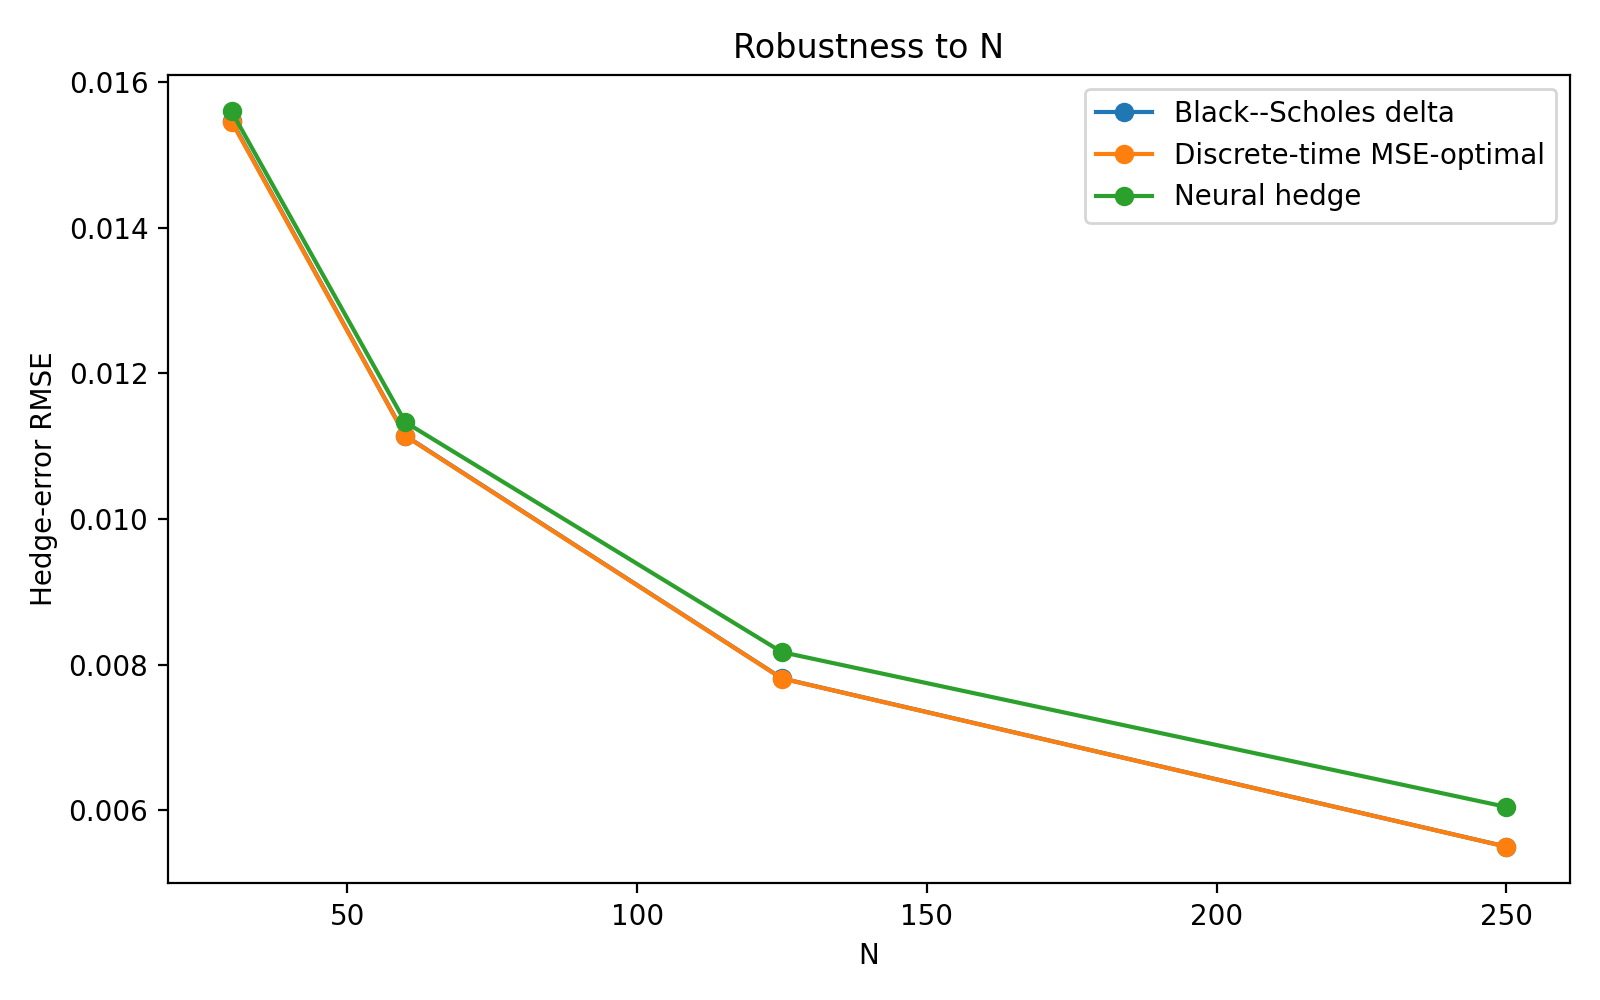
\includegraphics[
        width=\linewidth,
        height=4.6cm,
        keepaspectratio
    ]{sections/robustness_rmse_vs_N.png}
\end{column}
%---------------------------------------------------------
% RESULTS
%---------------------------------------------------------
\begin{column}{0.34\textwidth}
    \centering
    % ---- headline stat box ----
    \begin{tcolorbox}[
        colback=Teal!8,
        colframe=Teal,
        boxrule=0.4pt,
        arc=1.5pt,
        left=4pt,right=4pt,top=3pt,bottom=3pt,
        width=0.98\linewidth
    ]
    \centering
    {\footnotesize Mean neural-to-optimal RMSE ratio}\\[2pt]
    {\Large\bfseries\color{Teal} 1.049}\\[1pt]
    {\scriptsize (Range 1.009--1.099)}
    \end{tcolorbox}

    \vspace{0.22cm}

    \raggedright
    {\color{Teal}\scriptsize\(\blacktriangleright\)}\hspace{0.04cm}
    {\footnotesize Neural hedge remains at most \(10\%\) above the discrete-time optimum}

    \vspace{0.18cm}

    {\color{Teal}\scriptsize\(\blacktriangleright\)}\hspace{0.04cm}
    {\footnotesize Largest relative gap occurs at \(N=250\)}
\end{column}
\end{columns}
\end{frame}

\begin{frame}[t]{Generalisation Failure of the Single-Scenario Hedger}
\vspace{-0.18cm}
{\small
\begin{itemize}
    \setlength{\itemsep}{0pt}
    \item One model is trained at
    \((K^\ast,\sigma^\ast)=(0.9,0.4)\)
    and evaluated elsewhere \textbf{without retraining}.
\end{itemize}
}
\vspace{0.15cm} % pushes both graph and text down slightly
\begin{columns}[c,onlytextwidth]
%=================================================
% Graph
%=================================================
\begin{column}{0.60\textwidth} % widened slightly to make plot bigger
\centering
\vspace{0.35cm} % nudges the graph further down
\begin{tikzpicture}
\begin{axis}[
    width=\linewidth,
    height=5.4cm, % increased from 4.75cm
    ybar,
    bar width=7pt,
    ymin=0,
    ymax=320,
    ylabel={NN/DT RMSE ratio},
    ylabel style={font=\tiny},
    ytick={0,50,100,150,200,250,300},
    yticklabel style={font=\tiny},
    axis lines*=left,
    axis line style={color=black!65},
    ymajorgrids,
    grid style={color=black!15,line width=0.3pt},
    symbolic x coords={
        K0.9s0.4,
        K0.9s0.6,
        K1.1s0.6,
        K1.1s0.4,
        K0.9s0.2,
        K0.7s0.6,
        K1.1s0.2,
        K0.7s0.4,
        K0.7s0.2
    },
    xtick=data,
    xticklabels={
        {$0.9,0.4^\ast$},
        {$0.9,0.6$},
        {$1.1,0.6$},
        {$1.1,0.4$},
        {$0.9,0.2$},
        {$0.7,0.6$},
        {$1.1,0.2$},
        {$0.7,0.4$},
        {$0.7,0.2$}
    },
    xticklabel style={
        rotate=90,
        anchor=east,
        font=\tiny,
        inner sep=1pt
    },
    enlarge x limits=0.07,
    nodes near coords={
        \pgfmathprintnumber[
            precision=1,
            fixed
        ]{\pgfplotspointmeta}$\times$
    },
    every node near coord/.append style={
        font=\tiny,
        anchor=south
    },
    tick style={draw=none}
]
\addplot[
    ybar,
    fill=Teal!35,
    draw=none
] coordinates {
    (K0.9s0.6,4.8)
    (K1.1s0.6,7.8)
    (K1.1s0.4,14.1)
    (K0.9s0.2,14.3)
    (K0.7s0.6,24.7)
    (K1.1s0.2,39.3)
    (K0.7s0.4,40.6)
    (K0.7s0.2,291.3)
};
\addplot[
    ybar,
    fill=Teal,
    draw=none
] coordinates {
    (K0.9s0.4,1.0)
};
\end{axis}
\end{tikzpicture}
\vspace{-0.06cm}
{\tiny Horizontal axis: \((K,\sigma)\) combinations.}
\end{column}
%=================================================
% Reasons
%=================================================
\begin{column}{0.37\textwidth} % slightly narrowed to balance widened graph column
\vspace{0.35cm} % extra downward nudge for the text block
{\small\bfseries Why does it fail?}
\vspace{0.12cm}
{\footnotesize
\begin{enumerate}
    \setlength{\itemsep}{0.16cm}
    \setlength{\topsep}{0pt}
    \item \textbf{Single training scenario:}
    No variation from which to learn dependence on \(K\) or \(\sigma\).
    \item \textbf{Strike is hardcoded:}
    \(K^\ast\) is built into log-moneyness.
    \item \textbf{Volatility is missing:}
    The network has no input through which it can respond to a change
    in \(\sigma\).
\end{enumerate}
}
\end{column}
\end{columns}
\vspace{0.08cm}
\vspace{0.02cm}
\note{
Contrast this result with retraining.
When retrained at each setting, the architecture remains close to optimal.
When the same frozen network is moved to new settings, the error can rise
by roughly two orders of magnitude.
}
\end{frame}

\speakerlabel{Micaela}{1:30}

\begin{frame}[t]{The Parameter-Conditioned Hedger}

\vspace{-0.18cm}

%=================================================
% MODEL COMPARISON
%=================================================

\begin{center}

\renewcommand{\arraystretch}{1.28}
\setlength{\tabcolsep}{8pt}

{\small
\begin{tabular}{
    p{0.18\textwidth}
    p{0.35\textwidth}
    p{0.38\textwidth}
}
\toprule
&
\textbf{Original network}
&
\textbf{Conditioned network}
\\
\midrule

\textbf{Inputs}
&
\(\displaystyle
\left(
\log\frac{S}{K},
\frac{\tau}{T}
\right)\)
&
\(\displaystyle
\left(
\log\frac{S}{K},
\frac{\tau}{T},
K,\sigma
\right)\)
\\

\textbf{Training}
&
Fixed \(K=0.9,\ \sigma=0.4\)
&
\(K\sim U(0.7,1.1)\),\quad
\(\sigma\sim U(0.2,0.6)\)
\\

\textbf{Paths}
&
\(100\,000\)
&
\(200\,000\)
\\

\textbf{Premium}
&
Learned jointly
&
Analytic Black--Scholes premium
\\

\bottomrule
\end{tabular}
}

\end{center}

\vspace{0.20cm}

%=================================================
% RESULTS
%=================================================

\begin{columns}[T,onlytextwidth]

%-------------------------------------------------
% Interpolation
%-------------------------------------------------
\begin{column}{0.48\textwidth}

\centering
{\small\bfseries Interpolation}

\vspace{0.07cm}

{\footnotesize
Inside the training range
\[
K\in[0.7,1.1],
\qquad
\sigma\in[0.2,0.6].
\]
}

\vspace{-0.12cm}

{\footnotesize
\begin{itemize}
    \setlength{\itemsep}{0.11cm}

    \item Tested across nine parameter combinations.

    \item Maximum RMSE gap:\leq 0.00018



\end{itemize}
}

\end{column}

%-------------------------------------------------
% Extrapolation
%-------------------------------------------------
\begin{column}{0.48\textwidth}

\centering
{\small\bfseries Extrapolation}

\vspace{0.07cm}

{\footnotesize
Outside the training range
\[
K\in\{0.6,1.3\},
\qquad
\sigma\in\{0.1,0.8\}.
\]
}

\vspace{-0.12cm}

{\footnotesize
\begin{itemize}
    \setlength{\itemsep}{0.11cm}

    \item Strike extrapolation remains within \(0.00004\) of the
    optimum.

    \item Worst vol.\ gap at $\sigma=0.1$: $\approx 3\times$ the optimum.

\end{itemize}
}

\end{column}

\end{columns}

\vspace{0.04cm}




\vspace{0.01cm}

{\tiny\color{Slate}
Submitted report, Sec.\ 4.1.3 and Table 4.3.
}

\note{
Explain that the model is no longer tied to one contract.
Strike and volatility are now explicit inputs, and training covers a
continuous parameter range. The analytic premium is supplied to separate
pricing performance from hedging performance.
}

\end{frame}
